\documentclass[journal,transmag]{IEEEtran}

\usepackage{amsmath}
\usepackage{amssymb}
\usepackage{graphicx}
\usepackage{algpseudocode}
\usepackage{algorithm}
\usepackage{subfigure}
\usepackage{booktabs}
\usepackage{url}
\usepackage{breakurl}
%\usepackage{hyperref}
\usepackage[breaklinks]{hyperref}
\usepackage[table,xcdraw]{xcolor}
\usepackage{lmodern}
\usepackage[T1]{fontenc}
\usepackage{placeins}

\begin{document}

\def\UrlBreaks{\do\/\do-}

%
% paper title
% Titles are generally capitalized except for words such as a, an, and, as,
% at, but, by, for, in, nor, of, on, or, the, to and up, which are usually
% not capitalized unless they are the first or last word of the title.
% Linebreaks \\ can be used within to get better formatting as desired.
% Do not put math or special symbols in the title.
\title{CS27020 Assignment: Moma madness}


% author names and affiliations
% transmag papers use the long conference author name format.

\author{\IEEEauthorblockN{Lukasz Wrzolek}
\IEEEauthorblockA{Department of Computer Science, Aberystwyth University, Aberystwyth, SY23 3DB, UK}}% <-this % stops an unwanted space

% The paper headers
\markboth{CS27020-MOMA Madness}%
{L. Wrzolek}

\IEEEtitleabstractindextext{%

\begin{abstract}
\textit{This paper presents a novel approach to Modelling Databases. In this assignment I have been given a subset of this dataset in un-normalised form. My task was to understand the structure in this data and bring it up to 3NF, implement these 3NF relations in PostgreSQL, deliver an entity-relationship model, and execute some queries on this data. These activities I will described in this report which summarises and justifies the design and decisions I have made.    }
\end{abstract}

}

%make the title area
\maketitle

\IEEEdisplaynontitleabstractindextext

\onecolumn

\section{Introduction}

\IEEEPARstart{O}{ne} of the cool datasets that has been made freely available is from the New York based gallery MOMA. This Museum of Modern Art's collection dataset \url{https://github.com/MuseumofModernArt/collection} contains 126,101 records detailing some of the artwork held at New York's most famous art gallery. However, because we are dealing with artists rather than databasists, the dataset is in un-normalised form. Madness! \footnote{Introduction is modified version on Introduction from Assignment Description}

\section{Database Design}

This section describe design the database where I had to do normalisation, identify primary keys and bring database to third normal form. Although, I had to find functional dependencies for each attribute are identified to proceed the next stages of firs, second and third normal form.
\newline

\subsection {Primary keys and functional dependencies}


I have been given a sql file from university with data which contain a complete table moma in un-normalized form. 

I have listed the attributes of the moma table here:
\textbf{moma} (title, artist, artist\_bio, year, medium, dimensions, credit\_line, \underline{moma\_number}, classification, department, date\_acquired, curator\_approved, \underline{object\_id}, url)

\textbf{description of the attributes:}

\begin{itemize}
	\item title - The title of the work of art
	\item artist - the name and surname of the artist 
	\item artist\_bio - The artist information about date of birth, place and date of death 
	\item year - The production year of the art
	\item medium - the medium of the art
	\item dimensions - dimension of the art
	\item credit\_line - the company which gave that art for the museum
	\item moma\_number - it is the number of moma in database
	\item classification - it shows where the art has been located and in which department
	\item department - departments in moma
	\item date\_acquired  - the date when museum got that art
	\item curator\_approved - Y or N if the art is approved by curator or no
	\item object\_id - an unique id for the art
	\item URL - url address of that art ended by object\_id
\end{itemize}

The functional dependencies are desreibed below
\newline


\subsubsection {Functional dependencies}

In the above un-normalized form of the database I have found a few dependencies of the following  attributes:
 
$artist \rightarrow artist\_bio$

$artist\_bio \rightarrow artist$

Artist and artist\_bio is 1..1 dependency so that dependency goes in both ways.
\newline


$object\_id \rightarrow moma\_number$

$moma\_number \rightarrow object\_id$

This dependency is the same as artist and artist\_bio. Their relation is 1..1 so it will work in both ways
\newline


$object\_id \rightarrow url$

If URL exist at the end of the address we have an object\_id which separate different works of art
\newline

$object\_id \rightarrow (title, artist, artist\_bio, year, medium, dimensions, credit\_line, moma\_number, classification, department,$

$date\_acquired, curator\_approved, url)$

Object\_id determines pretty much everything, because as a primary key it has a unique value, so even if values are the same it doesnt matter because that value has relation (1..*) 
\newline

$moma\_number \rightarrow (title, artist, artist\_bio, year, medium, dimensions, credit\_line, classification, department,$ 

$date\_acquired, curator\_approved, object\_id, url)$
With moma\_number we have the same situation like in object\_id. The specific falues which determines multiple values i.e. title and artist are alright in functional dependencies
\newline

$(object\_id, moma\_number) \rightarrow (title, artist, artist\_bio, year, medium, dimensions, credit_line, classification, department,$

$date\_acquired, curator\_approved, url)$
\newline

\subsubsection {Primary Keys}

Working thtough the functional dependencies I spotted that object\_id and moma\_number are enough to find information about the work of art so I chase one of it to be a primary key of moma for un normalised form

\section {From UNF to 3NF: an account of the normalisation process}

Once the primary keys are identified and funcional dependencies are descreibed I was able to start normalisation the structure. 

\subsection {1st Normal Form}

First step of the normalisation process is identyfing the unique values. The candidate kyes are moma\_number and object\_id. Although, moma\_number is a candidate key it has records like 2605.2008.1-13, so taht record can be splitted for 13 different record and every of that record will be unique. The beginning of it will be 2605.2008. followed by number from 1 to 13. 
I have done the same for moma\_number by splitting it's tuples as I introduced before. After that moma\_number wasn't unique. It has two the same records:
\newline
\begin{enumerate}
\item "ETCHINGS FROM ECCLESIASTES" with moma number 30.1966.1-18
\item "ECCLESIASTES III:1 (plate, folio 10) from ETCHINGS FROM EC-CLESIASTES" with moma number 30.1966.4
\end{enumerate}

To avoid duplication in moma\_number I have created a query which finding a duplicated values and adding next number after "-" mark. In that process I created new relation called dimensions (\underline{dimension\_id}, moma\_number, dimensions, object\_id). I left touple object\_id in that relation because I want to know which dimension belong to the object. 
\newline

The next part of bringing structure to first normal form is removing the repeating units found in the un-normalized form along with any attributes that are functionally dependent on them. Doing so I splitted moma\_number, artist\_bio for a different, atomic values. I have created new attributes caalled (artist, nationality, birth\_date, death\_date), and splitted artist\_bio as a new four attributes. 
\newline

Next non atomic atribute is medium. I had multiple values so I had to create next relation media. After that I moved splitted media to new relation with obiect\_id and media\_id has been created which is a primary key of media relation. Next thing was creation the relation called "materials" and copying obiect\_id from "moma" relation. I set it up for a primary key in that table. Some of media values in "moma" relation has null values so not every value of obiect\_id will be in "media" relation. Thats why I chase to fill obiect\_id in "materials" relation from "moma" relation, to collect every value of that record. When I finished it I added touple media\_id to "materials" and filled it up from "media" relation, leaving <null> where obiect\_id didn't exist in "media" relation. When the separate id's from "media" table was collected with their object\_id's I dropped that touple from "media" relation. 

relation media (\underline{media\_id}, medium)

relation materials(\underline{object\_id},media\_id*,dimension\_id*)

relation dimensions(\underline{dimension\_id}, moma\_number, dimensions, object\_id)

\subsection {2nd Normal Form} 

When I brought my database to the first normal form, so my tuples has atomic values I created table artists $(\underline{artist}, nationality, birth\_date, death\_date)$. In relation "moma" artist value is not unique so, when I was transfering artists to their table I had to do it by using distinct keyword and artist touple became a primary key itself. 

Next relation created was classification (\underline{moma\_number}, classification, department, date\_acquired, curator\_approved, credit\_line). 

\subsection {3rd Normal Form}

Next step was to create a new relation classifications $(\underline{classification},department)$ to store classifications and their departments. There was a transitive dependency $title \rightarrow  department$, because if I know the title I have a moma\_number for it, following so I have classification and then I have department.
\newpage

\section {Implementation in postgres}

In this section I will describe step by step my proces of designing the database and my queries which I used to get form of the database.

\subsection {Artist process design}

First thing than needs to be done is set up the primary key for moma teble at un-normalised form. It will be object\_id as I wrote before. 
\newline

- -set up primary key for moma

ALTER TABLE moma ADD PRIMARY KEY (object\_id);
\newline

Next thing is creating new tuples in "moma" relation which gonna hold our splitted values.
\newline

- -create columns for new values

ALTER TABLE luw19.moma

ADD COLUMN nationality TEXT,

ADD COLUMN birth\_place TEXT,

ADD COLUMN birth\_date INTEGER,

ADD COLUMN death\_date INTEGER;
\newline

Now I was ready to write a query to split values and update moma relation
\newline

- - perform update moma table

WITH splitted\_data AS (

SELECT title,

       detail[1] AS nationality,

       detail[4] AS birth\_place,

       detail[5] AS birth\_date,

       detail[6] AS death\_date,

       object\_id

FROM (SELECT luw19.moma.*,

           $  regexp\_matches(luw19.moma.artist\_bio, '\backslash (([ \wedge ),]+),?\backslash s?(born )?(([\wedge \backslash .]+)\backslash .? )?(\backslash d\{4\})?(\backslash d\{4\})?\backslash )')$ AS detail

      FROM luw19.moma

     ) t

)

UPDATE luw19.moma

SET

  nationality = val.nationality,

  birth\_place = val.birth\_place,

  birth\_date = val.birth\_date :: INTEGER,

  death\_date = val.death\_date :: INTEGER

FROM (

       SELECT

         nationality,

         birth\_place,

         birth\_date,

         death\_date,

         object\_id

       FROM splitted\_data

     ) AS val

WHERE luw19.moma.object\_id = val.object\_id;
\newline

ALTER TABLE moma DROP artist\_bio;

\footnote{I am writing using latex so symbol $\wedge$ is really weird displayed and it can generate problems if somebody copy that code and use it in future. Make sure that you check it before!}
\newpage
Then moma relation look like this:

cs27020\_15\_16=> $\backslash$ d moma \ref{moma}
\begin{table}[]
\centering
\caption{luw19.moma}
\label{moma}
\begin{tabular}{c|c|c}
column            & type                    & modifiers \\ \hline
title             & character varying(800)  &           \\
artist            & character varying(100)  &           \\
year              & integer                 &           \\
medium            & character varying(1500) &           \\
dimensions        & character varying(2500) &           \\
credit\_line      & character varying(700)  &           \\
moma\_number      & character varying(20)   &           \\
classification    & character varying(100)  &           \\
department        & character varying(100)  &           \\
date\_acquired    & date                    &           \\
curator\_approved & character varying(1)    &           \\
object\_id        & integer                 & not null  \\
url               & character varying(200)  &           \\
nationality       & text                    &           \\
birth\_place      & text                    &           \\
birth\_date       & integer                 &           \\
dearth\_date      & integer                 &          
\end{tabular}
\end{table}
\footnote{I had to create the table from the output because, output wasn't clear. copied versions can be found here: \ref{bad}}

\subsection {Media}

Then I created media relation, and splitted medium by using delimeters and set first letter to capital to avoid duplicating records. 
\newline

- -creating table which will hold a media

CREATE TABLE materials (object\_id INTEGER, PRIMARY KEY (object\_id));

INSERT INTO materials(object\_id)

    SELECT object\_id FROM moma;

ALTER TABLE materials ADD COLUMN media\_id INTEGER;

- -creating and splitting media table

CREATE TABLE media (object\_id INTEGER,medium VARCHAR(1500));

- -inserting values

INSERT INTO media(object\_id,medium)

    SELECT object\_id,

      regexp\_split\_to\_table("medium", '(([,;] (?!printed))|[,;]? and )') "medium"

FROM luw19.moma;

- -adding a primary key for that table

ALTER TABLE media ADD COLUMN media\_id SERIAL PRIMARY KEY;

- -update materials from media

UPDATE materials

SET media\_id=media.media\_id

FROM media WHERE materials.object\_id=media.object\_id;

- -dropping object\_id

ALTER TABLE media DROP object\_id;
\newline

That query creates two relations: Materials \ref{materials} and media \ref{media}
\newline

cs27020\_15\_16=> $\backslash$ d materials \ref{materials}
\newline

\begin{table}[]
\centering
\caption{luw19.materials}
\label{materials}
\begin{tabular}{c|c|c}
Column        & Type    & Modifiers \\ \hline
obiect\_id    & integer & not null  \\
media\_id     & integer &           \\
dimension\_id & text    &          
\end{tabular}
\end{table}


Indexes:
    "materials\_pkey" PRIMARY KEY, btree (object\_id)
Foreign-key constraints:
    "materials\_dimensions\_dimension\_id\_fk" FOREIGN KEY (dimension\_id) REFERENCES dimensions(dimension\_id)
    "materials\_media\_media\_id\_fk" FOREIGN KEY (media\_id) REFERENCES media(media\_id)
Referenced by:
    TABLE "moma" CONSTRAINT "moma\_materials\_object\_id\_fk" FOREIGN KEY (object\_id) REFERENCES materials(object\_id)
\newline

cs27020\_15\_16=> $\backslash$ d media \ref{media}
\newline

\begin{table}[]
\centering
\caption{luw19.media}
\label{media}
\begin{tabular}{c|c|c}
Column    & Type                    & Modifiers                                                   \\ \hline
medium    & character varying(1500) &                                                             \\
media\_id & integer                 & not null default nextval('media\_media\_id\_seq'::regclass)
\end{tabular}
\end{table}

Indexes:
    "media\_pkey" PRIMARY KEY, btree (media\_id)
Referenced by:
    TABLE "materials" CONSTRAINT "materials\_media\_media\_id\_fk" FOREIGN KEY (media\_id) REFERENCES media(media\_id)

\subsection {Dimensions}

As I mentioned before dimensions which had "-" are splittend and putted to different relation. 

- - dimensions table with splitted dimensions as dimension\_id

CREATE TABLE dimensions

  AS
  - -splitting dimensions

WITH splitted\_dimension AS (

        SELECT luw19.moma.moma\_number

        , $regexp\_replace(moma.moma\_number, '([0-9\backslash.]+\backslash.)([0-9]+)-([0-9]+)', e'\backslash \backslash 1', e'g')$ AS dimension\_id

        , $regexp\_replace(moma.moma\_number, '([0-9\backslash.]+\backslash.)([0-9]+)-([0-9]+)', e'\backslash \backslash 2', e'g')$ AS dimension

        , $regexp\_replace(moma.moma\_number, '([0-9\backslash.]+\backslash.)([0-9]+)-([0-9]+)', e'\backslash \backslash3', e'g')$ AS object

        , moma.dimensions

        , moma.object\_id

        FROM luw19.moma

        )

  SELECT a1.moma\_number

       , a1.dimension\_id $\|$ generate\_series( a1.dimension::integer, a1.object::integer)::TEXT AS dimension\_id

       , a1.dimensions, a1.object\_id

FROM splitted\_dimension a1

WHERE a1.dimension <> a1.dimension\_id

UNION ALL

SELECT a0.moma\_number

        , a0.dimension\_id AS dimension\_id

        , a0.dimensions, a0.object\_id

FROM splitted\_dimension a0

WHERE a0.dimension = a0.dimension\_id;

- -selecting non-unique values and giving them a selected index

with stats as (

    SELECT "dimension\_id",

           "object\_id",

           row\_number() over (partition by "dimension\_id" order by object\_id) as rn

    FROM dimensions

)

UPDATE dimensions

   SET "dimension\_id" = CASE WHEN s.rn > 1 THEN s."dimension\_id"$ \|$ '-'$ \|$ s.rn

                   ELSE s."dimension\_id"

              END

  FROM stats s

 WHERE S."dimension\_id" = dimensions."dimension\_id"
  
 AND S."object\_id" = dimensions."object\_id";

- -adding dimension\_id column to materials

ALTER TABLE materials ADD COLUMN dimension\_id TEXT;
- -update column to hold dimension\_id

UPDATE materials

SET dimension\_id=dimensions.dimension\_id

FROM dimensions WHERE dimensions.object\_id=materials.object\_id;
\newline

cs27020\_15\_16=> $\backslash$ d dimensions \ref{dimensions}
\newline

\begin{table}[]
\centering
\caption{luw19.dimensions}
\label{dimensions}
\begin{tabular}{c|c|c}
Column        & Type                    & Modifiers \\ \hline
moma\_number  & character varying(20)   &           \\
dimension\_id & text                    & not null  \\
dimensions    & character varying(2500) &           \\
obiejct\_id   & integer                 &          
\end{tabular}
\end{table}


Indexes:
    "dimensions\_pkey" PRIMARY KEY, btree (dimension\_id)
Referenced by:
    TABLE "materials" CONSTRAINT "materials\_dimensions\_dimension\_id\_fk" FOREIGN KEY (dimension\_id) REFERENCES dimensions(dimension\_id)
\newline


\subsection{Artist Table}

Simple code to move artists and their details to the relation "artists"
\newline

- -creating artist table


CREATE TABLE artists (artist VARCHAR(100) PRIMARY KEY , nationality VARCHAR(100), birth\_place VARCHAR(100), birth\_date INTEGER, death\_date INTEGER);

INSERT INTO artists (artist, nationality, birth\_place, birth\_date, death\_date)

    SELECT DISTINCT artist,

      nationality,

      birth\_place,

      birth\_date,

      death\_date

        FROM luw19.moma;


- -dropping old values

ALTER TABLE luw19.moma


  DROP artist,

  DROP nationality,

  DROP birth\_date,

  DROP birth\_place,

  DROP death\_date;
\newline


cs27020\_15\_16=> $\backslash$ d artists \ref{artists}
\newline

\begin{table}[]
\centering
\caption{luw19.artists}
\label{artists}
\begin{tabular}{c|c|c}
Column       & Type                   & Modifiers \\ \hline
artist       & character varying(100) & not null  \\
nationality  & character varying(100) &           \\
birth\_place & character varying(100) &           \\
birth\_date  & integer                &           \\
death\_date  & integer                &          
\end{tabular}
\end{table}


Indexes:
    "artists\_pkey" PRIMARY KEY, btree (artist)
Referenced by:
    TABLE "moma" CONSTRAINT "moma\_artists\_artist\_fk" FOREIGN KEY (artist) REFERENCES artists(artist)
\newline



\subsection {Classifications}

And The last relation classifications to hold distinct classification separatelly.
\newline

- - creating table classifications for the distinct classifiacation

CREATE TABLE classifications (classification VARCHAR(100) PRIMARY KEY, department VARCHAR(100));

INSERT INTO classifications (classification, department)

    SELECT DISTINCT classification,department

      FROM classification;
\newline

cs27020\_15\_16=> $\backslash$ d classifications \ref {classifications}


\begin{table}[]
\centering
\caption{luw19.classifications}
\label{classifications}
\begin{tabular}{c|c|c}
Column         & Type                   & Modifiers \\ \hline
classification & character varying(100) & not null  \\
department     & character varying(100) &          
\end{tabular}
\end{table}


Indexes:
    "classifications\_pkey" PRIMARY KEY, btree (classification)
Referenced by:
    TABLE "classification" CONSTRAINT "classification\_classifications\_classification\_fk" FOREIGN KEY (classification) REFERENCES classifications(classification)
\newline


\subsection {Moma in 3rd NF}

Moma relation after all operations

cs27020\_15\_16=> $\backslash$ d moma \ref{moma2}
\newline


\begin{table}[]
\centering
\caption{luw19.moma}
\label{moma2}
\begin{tabular}{c|c|c}
Column                              & Type                                        & Modifiers            \\ \hline
title                               & character varying(800)                      &                      \\
artist                              & character varying(100)                      &                      \\
year                                & integer                                     &                      \\
medium                              & character varying(1500)                     &                      \\
\multicolumn{1}{l|}{credit\_line}   & \multicolumn{1}{l|}{character varying(700)} & \multicolumn{1}{l}{} \\
\multicolumn{1}{l|}{classification} & \multicolumn{1}{l|}{character varying(100)} & \multicolumn{1}{l}{} \\
date\_acquired                      & date                                        &                      \\
curatior\_approved                  & character varying(1)                        &                      \\
object\_id                          & integer                                     & not null             \\
url                                 & character varying(200)                      &                     
\end{tabular}
\end{table}



Indexes:
    "moma\_pkey" PRIMARY KEY, btree (object\_id)
Foreign-key constraints:
    "moma\_artists\_artist\_fk" FOREIGN KEY (artist) REFERENCES artists(artist)
    "moma\_classifications\_classification\_fk" FOREIGN KEY (classification) REFERENCES classifications(classification)
    "moma\_materials\_object\_id\_fk" FOREIGN KEY (object\_id) REFERENCES materials(object\_id)

\section {SQL Queries}

\subsection{Yoko Ono}
- - query to find a title and department for Yoko Ono.

WITH yoko AS (

SELECT title,object\_id

  FROM moma

  WHERE artist = 'Yoko Ono'

)

SELECT

    moma.title, classifications.department

FROM

    yoko

    INNER JOIN moma on moma.object\_id=yoko.object\_id

    INNER JOIN classifications ON moma.classification = classifications.classification;
\newline

and produced output is 10 rows table \ref{yoko} : 

\begin{table}[]
\centering
\caption{Yoko Ono}
\label{yoko}
\begin{tabular}{c|c}
title                                                                                          & department                      \\ \hline
Mend Piece for John from S.M.S. No. 5                                                          & Prints \&amp; Illustrated Books \\
No. 4 (Bottoms)                                                                                & Film                            \\
Instructions for Paintings                                                                     & Prints \&amp; Illustrated Books \\
Piece for Nam June Paik no. 1                                                                  & Prints \&amp; Illustrated Books \\
Grapefruit                                                                                     & Prints \&amp; Illustrated Books \\
Typescript for Do It Yourself Fluxfest Presents Yoko Ono \&amp; Dance Co.                      & Prints \&amp; Illustrated Books \\
Catalogue for Yoko Ono's exhibition This is Not Here at the Everson Museum, Syracuse, New York & Prints \&amp; Illustrated Books \\
Grapefruit                                                                                     & Prints \&amp; Illustrated Books \\
Part Painting/Series 5/to Tony Cox                                                             & Prints \&amp; Illustrated Books \\
Do It Yourself Fluxfest Presents Yoko Ono \&amp; Dance Co.                                     & Prints \&amp; Illustrated Books
\end{tabular}
\end{table}

\subsection{List of the artists}

I have tried to do b. part of 4th point but, I don't why the query is not working correctly.
\newline

SELECT  artist, count(*) AS works, array\_agg(distinct year order by year asc)

FROM (SELECT

  media\_id,

  department

FROM (SELECT media\_id, classification FROM materials

         LEFT JOIN moma ON materials.object\_id = moma.object\_id)

  AS media\_with\_classifications

  LEFT JOIN classifications ON media\_with\_classifications.classification = classifications.classification)t

JOIN artists ON moma.artist = artists.artist

  JOIN moma ON moma.object\_id=materials.object\_id

GROUP BY artist ORDER BY works DESC LIMIT 10;


\section{Entity Relationship Diagram}

In this section I will show a diagrams of relationship. One of them is produced by DataGrip IDE \ref{d1}, second is created by me using an online diagram creator \ref{d2}. 


\begin{figure}[t]
\centering
[Entity Relationship Diagram]{
		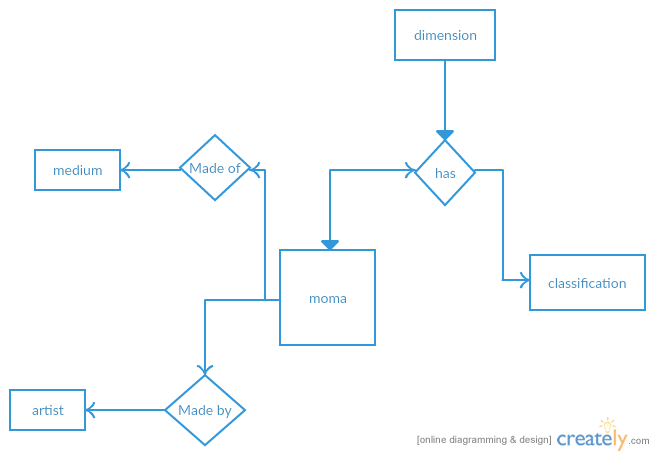
\includegraphics[width=1\textwidth]{diagram2.png}
	\label{d2}
	}
\end{figure}

\begin{figure*}[t]
\centering
	\subfigure[Diagram produced by DataGrip]{
		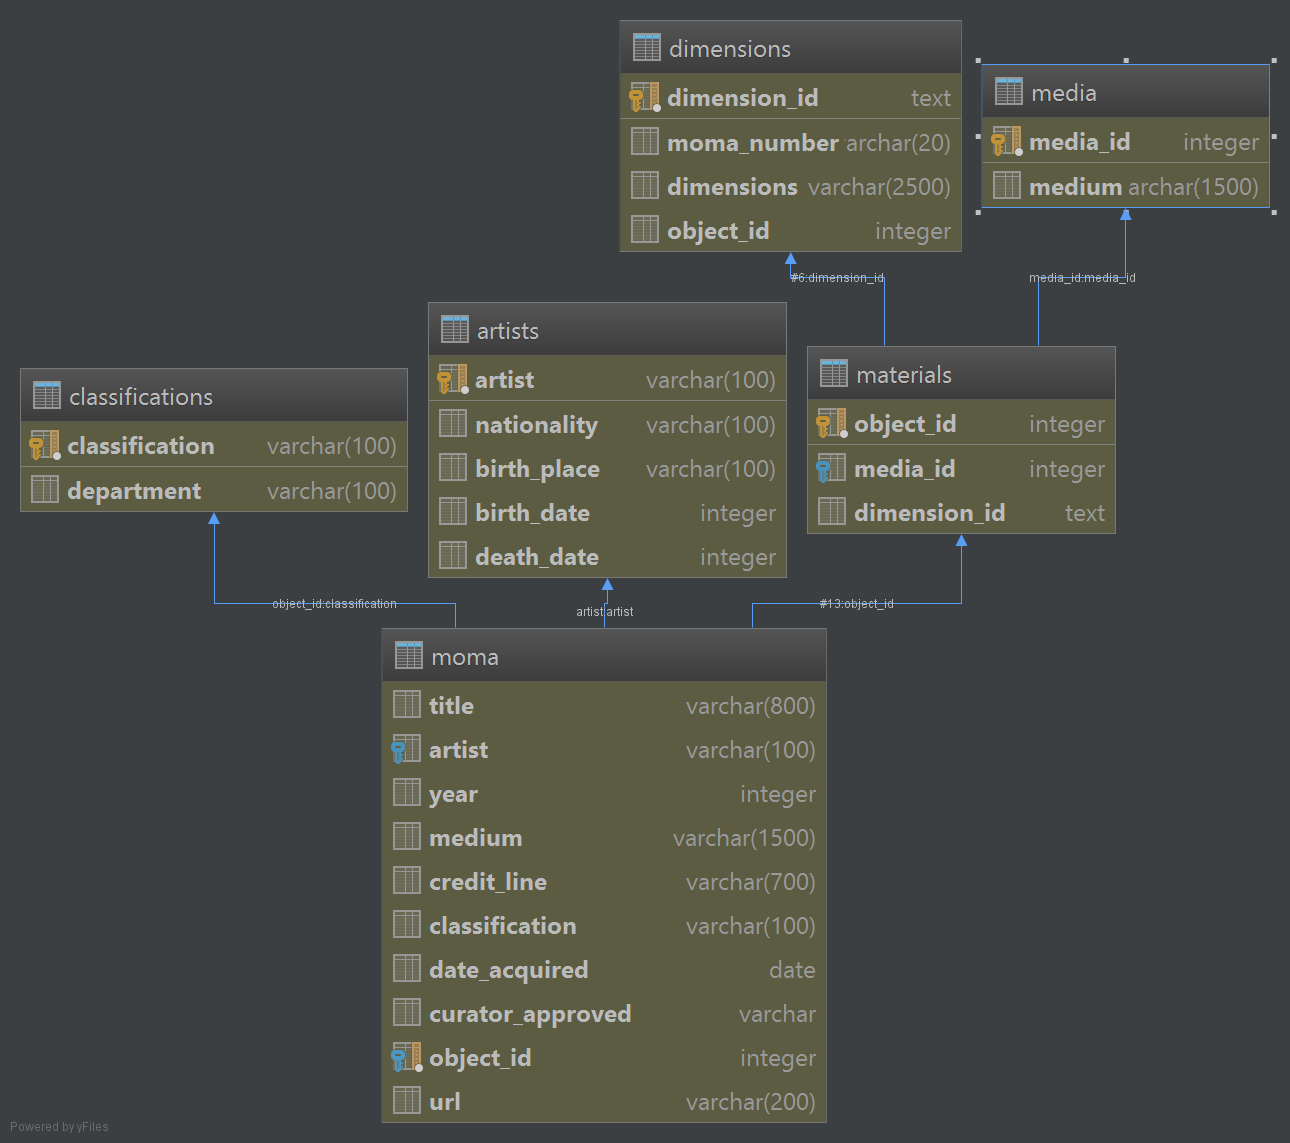
\includegraphics[width=1\textwidth,height = 15cm]{diagram.png}
	\label{d1}}
\label{diagram}
\end{figure*}


\section{Exploring MOMA further}

I have downloaded "extra.sql" from the page and run my script on it. The queries works good and created bigger database set than before. 

I have observed one interesting thing, namely is that I can work on the part of dataset from database, create a queries to design and sort out smaller database and after implement the same queries for the "parent" database with larger amount of information held. Although, on bigger dataset it takes much more time, so now I understand why is important do work on smaller sets of data







\clearpage
\newpage
\section {Copied versions from cmd}
\label{bad}

cs27020\_15\_16=> $\backslash$ d moma

Table "luw19.moma"

Column | Type | Modifiers
------------------+-------------------------+-----------
title | character varying(800) |
artist | character varying(100) |
year | integer |
medium | character varying(1500) |
dimensions | character varying(2500) |
credit\_line | character varying(700) |
moma\_number | character varying(20) |
classification | character varying(100) |
department | character varying(100) |
date\_acquired | date |
curator\_approved | character varying(1) |
object\_id | integer | not null
url | character varying(200) |
nationality | text |
birth\_place | text |
birth\_date | integer |
death\_date | integer |


Indexes:
"moma\_pkey" PRIMARY KEY, btree (object\_id)
\newline


cs27020\_15\_16=> $\backslash$ d materials

      Table "luw19.materials"

    Column    |  Type   | Modifiers
--------------+---------+-----------
 object\_id    | integer | not null
 media\_id     | integer |
 dimension\_id | text    |


Indexes:
    "materials\_pkey" PRIMARY KEY, btree (object\_id)
Foreign-key constraints:
    "materials\_dimensions\_dimension\_id\_fk" FOREIGN KEY (dimension\_id) REFERENCES dimensions(dimension\_id)
    "materials\_media\_media\_id\_fk" FOREIGN KEY (media\_id) REFERENCES media(media\_id)
Referenced by:
    TABLE "moma" CONSTRAINT "moma\_materials\_object\_id\_fk" FOREIGN KEY (object\_id) REFERENCES materials(object\_id)


cs27020\_15\_16=> $\backslash$ d media

                                      Table "luw19.media"
  Column  |          Type           |                        Modifiers          
----------+-------------------------+----------------------------------------------------------
 medium   | character varying(1500) |
 media\_id | integer                 | not null default nextval('media\_media\_id\_seq'::regclass)


Indexes:
    "media\_pkey" PRIMARY KEY, btree (media\_id)
Referenced by:
    TABLE "materials" CONSTRAINT "materials\_media\_media\_id\_fk" FOREIGN KEY (media\_id) REFERENCES media(media\_id)



cs27020\_15\_16=> $\backslash$ d dimensions


              Table "luw19.dimensions"
    Column    |          Type           | Modifiers
--------------+-------------------------+-----------
 moma\_number  | character varying(20)   |
 dimension\_id | text                    | not null
 dimensions   | character varying(2500) |
 object\_id    | integer                 |


Indexes:
    "dimensions\_pkey" PRIMARY KEY, btree (dimension\_id)
Referenced by:
    TABLE "materials" CONSTRAINT "materials\_dimensions\_dimension\_id\_fk" FOREIGN KEY (dimension\_id) REFERENCES dimensions(dimension\_id)


cs27020\_15\_16=> $\backslash$ d artists

              Table "luw19.artists"

   Column    |          Type          | Modifiers
-------------+------------------------+-----------
 artist      | character varying(100) | not null
 nationality | character varying(100) |
 birth\_place | character varying(100) |
 birth\_date  | integer                |
 death\_date  | integer                |


Indexes:
    "artists\_pkey" PRIMARY KEY, btree (artist)
Referenced by:
    TABLE "moma" CONSTRAINT "moma\_artists\_artist\_fk" FOREIGN KEY (artist) REFERENCES artists(artist)


cs27020\_15\_16=> $\backslash$ d classifications


            Table "luw19.classifications"

     Column     |          Type          | Modifiers
----------------+------------------------+-----------
 classification | character varying(100) | not null
 department     | character varying(100) |


Indexes:
    "classifications\_pkey" PRIMARY KEY, btree (classification)
Referenced by:
    TABLE "classification" CONSTRAINT "classification\_classifications\_classification\_fk" FOREIGN KEY (classification) REFERENCES classifications(classification)


cs27020\_15\_16=> $\backslash$ d moma


                   Table "luw19.moma"

      Column      |          Type           | Modifiers
------------------+-------------------------+-----------
 title            | character varying(800)  |
 artist           | character varying(100)  |
 year             | integer                 |
 medium           | character varying(1500) |
 credit\_line      | character varying(700)  |
 classification   | character varying(100)  |
 date\_acquired    | date                    |
 curator\_approved | character varying(1)    |
 object\_id        | integer                 | not null
 url              | character varying(200)  |


Indexes:
    "moma\_pkey" PRIMARY KEY, btree (object\_id)
Foreign-key constraints:
    "moma\_artists\_artist\_fk" FOREIGN KEY (artist) REFERENCES artists(artist)
    "moma\_classifications\_classification\_fk" FOREIGN KEY (classification) REFERENCES classifications(classification)
    "moma\_materials\_object\_id\_fk" FOREIGN KEY (object\_id) REFERENCES materials(object\_id)



















\end{document}